\chapter{Волны в волноводе}

Волновод -- это конструкция, которая позволяет волне переносить энергию внутри себя. С помощью неё можно протащить ЭМВ от их источника к приёмнику не рассеивая их попусту, а также делать другие странные вещи. Как правило волноводы бывают металлические (с металлической границей и диэлектрическим заполнением) и диэлектрические (как металлические, только без металла).

Рассмотрим простейший вариант волновода, а именно объём, ограниченный цилиндрической поверхностью. Направим ось \( Oz \) вдоль оси волновода. Тогда поля в волноводе будут иметь вид
\[
	\vec{E}(\vec{r}, t) = \vec{E}(\vec{r}_\perp)e^{i(\omega t - hz)},\quad
	\vec{H}(\vec{r}, t) = \vec{H}(\vec{r}_\perp)e^{i(\omega t - hz)}
\]
где \( h \) -- волноводное (продольное) волновое число.

Волна в волноводе удовлетворяет однородному волновому уравнению:
\[
	\square \vec{E}(\vec{r}, t) = 0,\quad \square = \Delta - \frac{1}{u^2}\ppder{}{t}.
\]
Подставляя вид поля, получаем
\[
	(\Delta_\perp - h^2 + \frac{\omega^2}{u^2}) \vec{E} = 0,
\]
где под \( \vec{E} \) понимается поле, зависящее только от поперечных координат. Везде далее в этой главе это будет подразумеваться. \( u \) -- скорость света в среде, заполняющей волновод.

Обозначим \( k = \omega / u \) -- постоянная распространения, \( g = \sqrt{k^2 - h^2} \) -- поперечное волновое число. Тогда уравнение примет вид уравнения Гельмгольца со всеми вытекающими решениями:
\[
	(\Delta_\perp + g^2) \vec{E} = 0, \quad (\Delta_\perp + g^2) \vec{H} = 0
\]
Вид этих решений зависит от выбора системы координат.

Отметим, что компоненты связаны друг с другом через уравнения Максвелла:
\[
	\begin{cases}
		\rotor\vec{E} = -i\omega\mu\vec{H},\\
		\rotor\vec{H} = i\omega\eps\vec{E},
	\end{cases}
\]

Выберем в каждой точке перпендикулярные единичные вектора \( \vec{e}_\xi \) и \( \vec{e}_\eta \) так, чтобы \( (\vec{e}_\xi, \vec{e}_\eta, \vec{e}_z) = 1 \) и введём вдоль них координаты \( \xi \) и \( \eta \). Это соответствует любым ортогональным координатам. Расписывая покоординатно, имеем
\[
	\begin{cases}
		\frac{1}{l_\eta}\pder{E_z}{\eta} + ih E_\eta = -i\omega\mu H_\xi,\\
		-\frac{1}{l_\xi}\pder{E_z}{\xi} - ih E_\xi = -i\omega\mu H_\eta,\\
		\frac{1}{l_\eta}\pder{H_z}{\eta} + ihH_\eta = i\omega\eps E_\xi,\\
		-\frac{1}{l_\xi}\pder{H_z}{\xi} - ihH_\xi = i\omega\eps E_\eta,\\
	\end{cases}
\]
где \( l_\alpha \) -- коэффициенты Ламэ (буква \( H \) занята магнитным полем).

Можно рассматривать поперечные компоненты как функции продольных:
\[
	\begin{cases}
		ihE_\eta + i\omega\mu H_\xi = -\frac{1}{l_\eta}\pder{E_z}{\eta},\\
		i\omega\eps E_\eta + ihH_\xi = -\frac{1}{l_\xi}\pder{H_z}{\xi},\\
		-ihE_\xi + i\omega\mu H_\eta = \frac{1}{l_\xi}\pder{E_z}{\xi},\\
		- i\omega\eps E_\xi + ihH_\eta = -\frac{1}{l_\eta}\pder{H_z}{\eta},\\
	\end{cases}
\]
откуда
\[
	\begin{cases}
		E_\xi  = \frac{-i}{g^2}\left(\frac{h}{l_\xi}\pder{E_z}{\xi} +\frac{\omega\mu}{l_\eta}\pder{H_z}{\eta}\right),\\
		E_\eta = \frac{-i}{g^2}\left(\frac{h}{l_\eta}\pder{E_z}{\eta} - \frac{\omega\mu}{l_\xi}\pder{H_z}{\xi}\right),\\
		H_\xi  = \frac{i}{g^2}\left(\frac{\omega\eps}{l_\eta}\pder{E_z}{\eta} - \frac{h}{l_\xi}\pder{H_z}{\xi}\right),\\
		H_\eta = \frac{-i}{g^2}\left(\frac{\omega\eps}{l_\xi}\pder{E_z}{\xi} + \frac{h}{l_\eta}\pder{H_z}{\eta}\right),
	\end{cases}
\]
а \( E_z \) и \( H_z \) -- решения уравнений Гельмгольца:
\[
	(\Delta_\perp + g^2) E_z = 0, \quad (\Delta_\perp + g^2) H_z = 0
\]

Для полной постановки задачи осталось определить граничные условия.

\section{В прямоугольном волноводе}

\begin{gather*}
	E_x = \frac{-i}{g^2}\left(h\pder{E_z}{x} + \omega\mu\pder{H_z}{y}\right),\\
	E_y = \frac{-i}{g^2}\left(h\pder{E_z}{y} - \omega\mu\pder{H_z}{x}\right),\\
	H_x = \frac{i}{g^2}\left(\omega\eps\pder{E_z}{y} - h\pder{H_z}{x}\right),\\
	H_y = \frac{-i}{g^2}\left(\omega\eps\pder{E_z}{x} + h\pder{H_z}{y}\right).
\end{gather*}

В системе могут существовать отдельные TE и TM волны, если на контуре волновода
\[
	\pder{E_z}{l} = \pder{H_z}{l} = 0.
\]
Если условие не выполняются, то в системе будут наблюдаться гибридные волны.

Рассмотрим прямоугольный волновод \( a \times b, a > b, a || Ox \).

E-волны (TM) имеют в нём следующий вид:

\begin{align*}
	& E_z = E_0\sin\frac{m\pi x}{a}\sin\frac{n\pi y}{b},\\
	& H_z = 0,\\
	& E_x = -i\frac{hm\pi}{g_{m,n}^2a}E_0\cos\frac{m\pi x}{a}\sin\frac{n\pi y}{b},\\
	& E_y = -i\frac{hn\pi}{g_{m,n}^2b}E_0\sin\frac{m\pi x}{a}\cos\frac{n\pi y}{b},\\
	& H_x = -\frac{\omega\eps}{h}E_y = i\frac{\omega\eps n\pi}{g_{m,n}^2b}E_0
	 								\sin\frac{m\pi x}{a}\cos\frac{n\pi y}{b},\\
	& H_y = \frac{\omega\eps}{h}E_x = -i\frac{\omega\eps m\pi}{g_{m,n}^2a}E_0
	 								\cos\frac{m\pi x}{a}\sin\frac{n\pi y}{b}.
\end{align*}

H-волны (TE):
\begin{align*}
	& E_z = 0,\\
	& H_z = H_0\cos\frac{m\pi x}{a}\cos\frac{n\pi y}{b},\\
	& E_x = i\frac{\omega\mu n\pi}{g_{m,n}^2b}H_0\cos\frac{m\pi x}{a}\sin\frac{n\pi y}{b},\\
	& E_y = -i\frac{\omega\mu m\pi}{g_{m,n}^2a}H_0\sin\frac{m\pi x}{a}\cos\frac{n\pi y}{b},\\
	& H_x = -\frac{h}{\omega\mu}E_y = i\frac{hm\pi}{g_{m,n}^2a}H_0
	 								\sin\frac{m\pi x}{a}\cos\frac{n\pi y}{b},\\
	& H_y = \frac{h}{\omega\mu}E_x = -i\frac{h n\pi}{g_{m,n}^2b}H_0
	 								\cos\frac{m\pi x}{a}\sin\frac{n\pi y}{b}.
\end{align*}

Здесь \( g_{m,n} \) -- поперечное волновое число, определяемое выражением
\[
	g_{m,n} = \pi\sqrt{\frac{m^2}{a^2} + \frac{n^2}{b^2}}.
\]

Так как
\[
	h^2 = \beta^2 - g_{m,n}^2,
\]
то для данного типа волны существует критическая частота, ниже которой эта волна возбуждаться не может. Она называется критической:
\[
	\omega_c = \frac{c}{\sqrt{\eps_r \mu_r}}g_{m,n}.
\]

Дисперсионное соотношение имеет вид:
\[
	h^2 = \frac{\omega^2 \eps_r \mu_r}{c^2} - g_{m,n}^2,
\]
откуда
\[
	v_p = \frac{\omega}{h} = \frac{c}{\sqrt{\eps_r\mu_r}}\frac{1}{\sqrt{1 - \omega_c^2 / \omega^2}},
\]

\[
	v_g = \der{\omega}{h} = \frac{c}{\sqrt{\eps_r\mu_r}}\sqrt{1 - \omega_c^2 / \omega^2}.
\]

Заметим, что
\[
	v_p v_g = \frac{c^2}{\eps_r\mu_r} \text{ --- квадрат скорости света в среде.}
\]

\begin{center}
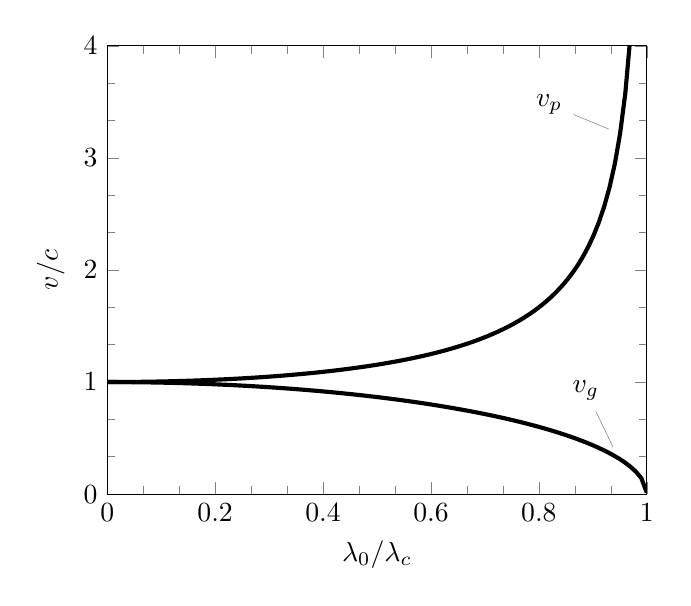
\begin{tikzpicture}
\begin{axis}[
	xmin = 0, xmax = 1, ymin = 0, ymax = 4,
    xlabel = {$\lambda_0 / \lambda_c$},
    ylabel = {$v / c$},
    minor tick num = 2
]
\addplot[domain=0:0.97,samples=100,line width=1.5pt]{(1 - x^2)^-0.5} node[pos=0.75,pin=170:{$v_p$}]{};
\addplot[domain=0:1,samples=100,line width=1.5pt]{sqrt(1 - x^2)} node[pos=0.8,pin=100:{$v_g$}]{};
\end{axis}
\end{tikzpicture}
\end{center}


Относительное расположение критических длин волн:
\begin{center}
	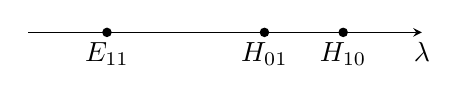
\begin{tikzpicture}[>=stealth]
		\draw[->](0,0) -- (5,0);
		\draw[fill] (1,0) circle(1.5pt) node[below]{$E_{11}$};
		\draw[fill] (3,0) circle(1.5pt) node[below]{$H_{01}$};
		\draw[fill] (4,0) circle(1.5pt) node[below]{$H_{10}$};
		\draw (5,0) node[below]{$\lambda$};
	\end{tikzpicture}
\end{center}

Характеристические сопротивления для волн:
\begin{align*}
	Z_c^E = & \sqrt{\frac{E_xE_x^* + E_yE_y^*}{H_xH_x^* + H_yH_y^*}} = \frac{h}{\omega\eps} = Z_c\sqrt{1 - \frac{\lambda_0^2}{\lambda_c^2}},\\
	Z_c^H = & \sqrt{\frac{E_xE_x^* + E_yE_y^*}{H_xH_x^* + H_yH_y^*}} = \frac{\omega\mu}{h} = \frac{Z_c}{\sqrt{1 - \frac{\lambda_0^2}{\lambda_c^2}}}.
\end{align*}

Рассмотрим передачу мощности в волне \( H_{10} \):
\[
	\Pi_z = -\frac{1}{2}E_y H_x^* = \frac{1}{2}\frac{h}{\omega\mu}E_yE_y^* = \frac{h}{2\omega\mu}\omega^2\mu^2 H_0^2\sin^2\frac{\pi x}{a} = \frac{\omega\mu h}{2}H_0^2\sin^2\frac{\pi x}{a},
\]
\[
	h= \frac{2\pi}{\lambda_0}\sqrt{1 - \frac{\lambda_0^2}{4a^2}},
\]
\[
	\Pi_z = \frac{\mu ca^2}{\pi\lambda_0^2}\sqrt{1 - \frac{\lambda_0^2}{4a^2}}H_0^2\sin^2\frac{\pi x}{a},
\]
а передаваемая мощность определяется интегралом по поперечному сечению:
\[
	P = \frac{\mu ca^3b}{2\pi\lambda_0^2}\sqrt{1 - \frac{\lambda_0^2}{4a^2}}H_0^2 = \frac{abh}{4\omega\mu}E_{max}^2.
\]


\section{Затухание}
Причины:
\begin{itemize}
	\item потери с среде
	\item потери в металле
	\item излучение в пространство
\end{itemize}

Чтобы учесть потери можно рассмотреть
\[
	h = h' - ih''
\]

Мощность потерь
\[
	P = P_d + P_m + P_e,
\]

Поверхностный ток на стенках волновода
\[
	\vec{i}_s = \vec{n}\times\vec{H}_\tau.
\]

Для потерь вдоль волновода имеет место соотношение
\[
	\der{P}{z} = -2h''P = -\der{P_m}{z}.
\]

\[
	\der{P}{z} = -\frac{1}{2}\Re Z_{Me}\oint_C |H_\tau^2| dl,
\]

\[
	h'' = \frac{1}{2}\frac{\Re Z_{Me}\oint_C |H_\tau^2| dl}{\iint_S \Pi_z dS}.
\]

\[
	\oint_C |H_\tau^2| dl = 2 \left( \int_{y=0, x=0}^{x=a} H_x^2 dx +
	\int_{x=0, y=0}^{y=b} H_y^2 dx  \right).
\]

\[
\int_{y=0, x=0}^{x=a} H_x^2 dx = \left(\frac{\omega\eps n\pi}{g_{m,n}^2b}\right)^2\int_{y=0, x=0}^{x=a} E_0^2\sin^2\frac{m\pi x}{a} dx = \frac{a}{2}\left(\frac{\omega\eps n\pi E_0}{g_{m,n}^2b}\right)^2.
\]
\[
	\int_{x=0, y=0}^{y=b} H_y^2 dx = \frac{b}{2}\left(
	\frac{\omega\eps m\pi}{g_{m,n}^2a}E_0\right)^2,
\]
\[
	\oint_C |H_\tau^2| dl =\left(\frac{\omega\eps \pi}{g_{m,n}^2}E_0\right)^2 \frac{n^2a^3 + m^2b^3}{a^2b^2}.
\]
Знаменатель:
\[
	\iint_S (E_xH_y^* - E_yH_x^*) dS = \frac{\omega\eps}{h}
	\left(\frac{h\pi}{g_{m,n}^2}E_0\right)^2\frac{ab}{4}
	\left(\frac{m^2}{a^2}+\frac{n^2}{b^2}\right) =
	\frac{\omega\eps}{h}
	\left(\frac{h}{g_{m,n}}E_0\right)^2\frac{ab}{4},
\]
откуда
\[
	h'' = \frac{2Z_{Me}\frac{\omega\eps \pi^2}{g_{m,n}^2} (n^2a^3 + m^2b^3)}{ha^3b^3}
\]

Если ввести сквозную нумерацию гармоник, то
\[
	\int (\vec{E}_m\times\vec{H}_n^*)\cdot\vec{dS}_\perp = \delta_{mn}N_m.
\]

Рассмотрим подробнее
\[
	(\vec{E}_m\times\vec{H}_n^*)\cdot\vec{z}_0 =
	\begin{vmatrix}
		E_{mx} & E_{my}\\
		H_{nx}^* & H_{ny}^*\\
	\end{vmatrix}
	=
	E_{mx}H_{ny}^* - E_{my}H_{nx}^*.
\]

Моды являются собсвенными функциями системы уравнений
\[
	\Delta_\perp E_{m\alpha} + g_m^2 E_{m\alpha} = 0,\quad \Delta_\perp H_{n\alpha}^* + g_n^2 H_{n\alpha}^* = 0.
\]
с нужными граничными условиями.

Помножим некоторые уравнения, чтобы получить:
\[
	H_{ny}^*\Delta_\perp E_{mx} + g_m^2 H_{ny}^*E_{mx} = 0,
\]
\[
	H_{nx}^*\Delta_\perp E_{my} + g_m^2 H_{nx}^*E_{my} = 0,
\]
откуда
\[
	g_m^2(E_{mx}H_{ny}^* - E_{my}H_{nx}^*) = H_{nx}^*\Delta_\perp E_{my} - H_{ny}^*\Delta_\perp E_{mx}
\]
Аналогично
\[
	g_n^2(E_{mx}H_{ny}^* - E_{my}H_{nx}^*) = \Delta_\perp H_{nx}^* E_{my} - \Delta_\perp H_{ny}^* E_{mx}
\]

Теперь:
\begin{align*}
	&(g_m^2 - g_n^2)(E_{mx}H_{ny}^* - E_{my}H_{nx}^*) =\\
	& = \int_{S_\perp} dS \left( H_{nx}^*\Delta_\perp E_{my} - \Delta_\perp H_{nx}^* E_{my} \right)
	-
	\int_{S_\perp} dS \left( H_{ny}^*\Delta_\perp E_{mx} - \Delta_\perp H_{ny}^* E_{mx} \right) =\\
	& = \int_C dl \left(H_{nx}^* \pder{E_{my}}{n} - E_{my}\pder{H_{ny}^*}{n}\right) -
	\int_C dl \left( H_{ny}^*\pder{E_{mx}}{n} - \pder{H_{ny}^*}{n} E_{mx} \right)
\end{align*}

\section{Коаксиальный волновод}
\begin{gather*}
	E_r =    \frac{-i}{g^2}\left(h\pder{E_z}{r} + \frac{\omega\mu}{r}\pder{H_z}{\phi}\right),\\
	E_\phi = \frac{-i}{g^2}\left(\frac{h}{r}\pder{E_z}{\phi} - \omega\mu\pder{H_z}{r}\right),\\
	H_r =    \frac{i}{g^2}\left(\frac{\omega\eps}{r}\pder{E_z}{\phi} - h\pder{H_z}{r}\right),\\
	H_\phi = \frac{-i}{g^2}\left(\omega\eps\pder{E_z}{r} + \frac{h}{r}\pder{H_z}{\phi}\right).
\end{gather*}

Основной режим работы -- TEM-волны, волноводные гармоники -- паразитные.

\[
	\Delta_\perp E_z = g^2 E_z = 0,\quad \Delta_\perp H_z = g^2 H_z = 0.
\]
с граничными
\[
	\left.E_\tau\right|_{r=a,b} = 0 \Rightarrow \left.E_z\right|_{r=a,b} = 0, \left.\pder{H_z}{r}\right|_{r=a,b} = 0
\]
\[
	\frac{1}{r}\pder{}{r}\left( rE_z \right) + \frac{1}{r^2}\ppder{E_z}{\phi} + g^2E_z = 0.
\]
\[
	E_z = [AJ_m(gr) + BN_m(gr)]\cos(m\phi)
\]
При \( b = 0 \) \( B = 0 \)
\[
	E_z = E_0J_m(gr)\cos(m\phi).
\]
Поперечные волновые числа определяются из условия
\[
	J_m(ga) = 0,\ g_{mn} = \frac{\nu_{mn}}{a}.
\]

\begin{align*}
	E_z &= E_0 J_m(\frac{\nu_{mn}}{a}r)\Phi(m\phi),\\
	E_r &= -\frac{iha}{\nu_{mn}}E_0 J_m'(\frac{\nu_{mn}}{a}r)\Phi(m\phi),\\
	E_\phi &= -\frac{iha^2m}{\nu_{mn}^2r}E_0 J_m(\frac{\nu_{mn}}{a}r)\Phi'(m\phi),\\
	H_z &= 0,\\
	H_r &= -\frac{\omega\eps}{h}E_\phi,\\
	H_\phi &= \frac{\omega\eps}{h}E_r.
\end{align*}


Рассмотрим теперь \( H \)-волны:
\[
	\Delta_\perp H_z + g^2H_z = 0,\quad \left.\pder{H_z}{n}\right|_{r=a,b}= 0
\]

\[
	H_z = [AJ_m(gr) + BN_m(gr)]\Phi(m\phi)
\]

Если \( b=0 \), то в силу ограниченности поля \(B = 0\), а дисперсионное соотношение имеет вид
\[
	J_m'(ga) = 0 \Rightarrow ga = \mu_{mn}, g_{mn} = \frac{\mu_{mn}}{a}, \lambda_c = \frac{2\pi a}{\mu_{mn}}, \mu_{11} = 1.841.
\]

Поля в волноводе имеют вид:
\begin{align*}
	H_z &= H_0 J_m(\frac{\mu_{mn}}{a}r)\Phi(m\phi),\\
	E_r &= -\frac{i\omega\mu a^2m}{r\mu_{mn}^2}H_0 J_m(\frac{\mu_{mn}}{a}r)\Phi'(m\phi),\\
	E_\phi &= \frac{i\omega\mu a}{\mu_{mn}}E_0 J_m'(\frac{\mu_{mn}}{a}r)\Phi(m\phi),\\
	E_z &= 0,\\
	H_r &= -\frac{h}{\omega\mu}E_\phi,\\
	H_\phi &= \frac{h}{\omega\mu}E_r.
\end{align*}

Для коаксиального волновода имеем
\[
	\begin{cases}
		AJ_m'(gb) + BN_m'(gb) = 0,\\
		AJ_m'(ga) + BN_m'(ga) = 0.\\
	\end{cases},
	\quad
	J_m'(gb)N_m'(ga) - J_m'(ga)N_m'(gb) = 0
\]

Характеристическое сопротивление волновода
\[
	Z_c = \frac{E_\perp}{H_\perp}.
\]

Рассчитаем потери в круглом волноводе (на гармонике \(E_{01}\)):
\[
	h'' = \frac{\Re Z_m}{2}\frac{\oint dl |\vec{H_\tau}|^2}{\iint \vec{dS}\cdot(\vec{E}\times\vec{H}^*)},
\]
\begin{align*}
	E_r &= -\frac{iha}{\nu_{01}}E_0 J_0'(\frac{\nu_{01}}{a}r),\\
	H_\phi &= \frac{\omega\eps}{h}E_r.
\end{align*}
\[
	\oint dl |\vec{H_\tau}|^2 = \int_0^{2\pi} a d\phi\,|H_\phi|^2 =
	\frac{a^3\omega^2\eps^2}{\nu_{01}^2}E_0^2J_0'^2(\nu_{01})\int_0^{2\pi} d\phi = \frac{2\pi a^3\omega^2\eps^2}{\nu_{01}^2}E_0^2J_0'^2(\nu_{01})
\]

\[
	\iint \vec{dS}\cdot(\vec{E}\times\vec{H}^*) = \int_0^{2\pi}d\phi\int_0^a rdr \frac{ha^2\omega\eps}{\nu_{01}^2}E_0^2J_0'^2(\frac{\nu_{01}}{a}r)= \frac{2\pi ha^2\omega\eps}{\nu_{01}^2}E_0^2 \int_0^a rdrJ_0'^2(\frac{\nu_{01}}{a}r)
\]
Рассмотрим подробнее интеграл:
\[
	\int_0^a rdr J_0'^2(\frac{\nu_{01}}{a}r) =
	\frac{a^2}{\nu_{01}^2}\int_0^{\nu_{01}} J_0'^2(x) x dx =
	\frac{a^2}{2}J_0'^2(\nu_{01}).
\]
Собирая всё вместе, получаем:
\[
	h'' = \frac{\Re Z_m}{2}\frac{\frac{2\pi a^3\omega^2\eps^2}{\nu_{01}^2}E_0^2J_0'^2(\nu_{01})}{\frac{2\pi ha^2\omega\eps}{\nu_{01}^2}E_0^2\frac{a^2}{2}J_0'^2(\nu_{01})} = \frac{\Re Z_m}{2}\frac{\omega\eps}{ha}.
\]

Определить число мод, возбуждаемых в волноводе 72 на 34 мм на частоте 10 ГГц.

Определить структуру токов в стенках волновода.

Определить размер квадратного волновода, если на частоте 7.5 ГГц фазовая скорость волны \(E_{21}\) равна \( u = 2.5c \).
\[
	g^2 = \pi^2\frac{n^2 + m^2}{a^2} = \omega^2/c^2 - h^2 = 4\pi^2f^2/c^2 \frac{5.25}{6.25},\ a^2 = \frac{6.25 c^2}{5.25}\frac{n^2 + m^2}{4f^2},
\]
\[
	a = \sqrt{\frac{6.25}{5.25}}\frac{c\sqrt{n^2 + m^2}}{2f} = 0.049~\text{м}.
\]

\section{Волноводы странной формы}

П-образные волноводы позволяют получать разреженный спектр. Расплатой за это является меньшая мощность и большие потери.

Для расчёта такого рода волноводов приходится использовать численные методы.


\section{Диэлектрические волноводы}

Рассмотрим оптически более плотный волновод в среде. В силу явления полного внутреннего отражения в нём может распространяться волна.

\[
	\sin\phi_0 = n_1 / n_2.
\]

При таких переотражениях получается волна, распространяющаяся вдоль волновода.

Фазовая скорость волны равна
\[
	v_p = \frac{u_2}{\sin\phi} \le u_1,
\]
\[
	u_1 \ge v_p \ge u_2.
\]

Угол \( \phi \) падения связан с размерами и частотой волны. Если \( \phi < \phi_0 \), то волна рассеивается в окружающее пространство. Следовательно, получается отсечка.

\[
	h^2 = k_1^2 - g_1^2 = k_2^2 - g_2^2.
\]
\[
	g_2^2 > 0,\ g_1^2 < 0,
\]
\[
	g_1 = iq,\ g_2 = g.
\]

\[
	\eps_1\mu_1\omega^2 + q^2 = \eps_2\mu_2\omega^2 - g^2.
\]
Пусть \( a \) -- характерный размер волновода, тогда
\[
	\overline{g} = ag,\quad \overline{q} = aq,
\]
\[
	\overline{q}^2 + \overline{g}^2 = a^2\omega^2\eps_1\mu_1(\overline{eps}\overline{\mu} - 1) = \overline{k}_1^2(\overline{eps}\overline{\mu} - 1) = \overline{R}^2.
\]
\(\overline{R}\) -- нормированная частота.